\documentclass[12pt]{article}
\usepackage{amsmath,amssymb,epsfig,bbm,capt-of,ifthen,calc}

%%%%%%%%%% Start TeXmacs macros
\newcommand{\tmfloatcontents}{}
\newlength{\tmfloatwidth}
\newcommand{\tmfloat}[5]{
  \renewcommand{\tmfloatcontents}{#4}
  \setlength{\tmfloatwidth}{\widthof{\tmfloatcontents}+1in}
  \ifthenelse{\equal{#2}{small}}
    {\ifthenelse{\lengthtest{\tmfloatwidth > \linewidth}}
      {\setlength{\tmfloatwidth}{\linewidth}}{}}
    {\setlength{\tmfloatwidth}{\linewidth}}  \begin{minipage}[#1]{\tmfloatwidth}
    \begin{center}
      \tmfloatcontents
      \captionof{#3}{#5}
    \end{center}
  \end{minipage}}
\newcommand{\tmem}[1]{{\em #1\/}}
\newcommand{\tmop}[1]{\operatorname{#1}}
\newcommand{\tmname}[1]{\textsc{#1}}
%%%%%%%%%% End TeXmacs macros

\begin{document}
\title{Dealing with Discontinuities}
\author{Michael Peters}
\date{\today}
\maketitle

\section{Introduction}
The Lagrangian method for solving maximization problems that we have studied
so far is sometimes the only way to get insight into the solution to your
problem. Most of the time, it is only part of the technique you need. The
reason is that the constraint sets consumers face often come with built-in
discontinuities of various sorts. You will see these every day. Your phone
company offers 100 minutes of long distance calling for a fixed fee, but if
you talk for more than 100 minutes, you pay big time. The local restaurant runs
a burger-beer special  \$ 6 for a burger and beer - and charges \$5 for each additional beer. Buy one issue of \textit{The Economist} magazine, and the price is about  \$ 5;
buy a year's subscription, and the price falls to about \$2 per issue.

To solve problems like these, you need to use a variety of different
techniques in combination. When approaching a problem, you may be tempted to simply
write down the Lagrangian, derive all the first order conditions, and
then, try to solve. This chapter is a warning that this will fail in most of
the problems you are likely to encounter. You will need the Lagrangian method,
but only as part of a larger toolbox.

Again, you may be tempted to rush to the `write down the first order conditions' 
approach--especially during an exam when time pressure keeps you from being your most
creative--but this is the wrong way to start in most situations. I am a big fan of
graphical methods for guessing the solution to problems. They are usually the
most useful at helping you to see the special properties of the problem you
are trying to solve. In a previous chapter, we solved a consumer's problem
using Lagrangian methods, where preferences were given by
\begin{equation}
  \text{$u ( x, y ) = x^{\alpha} y^{1 - \alpha} \label{cd}$}
\end{equation}
Graphical methods would start with a picture like the one you saw so much in
your first-year course.

\tmfloat{h}{small}{figure}{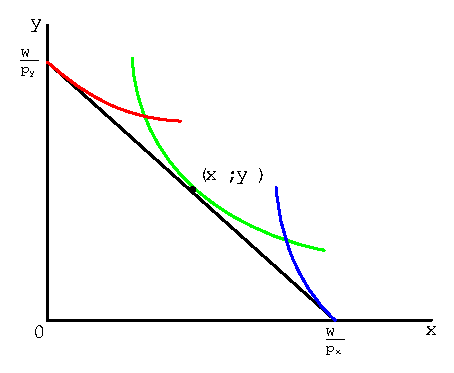
\epsfig{file=discontinuities_fig1.eps}}{\label{three}}

The best bundle for the consumer to choose is the one that lies on the highest
indifference curve that just touches the budget set. This indifference curve
could look like the green curve in Figure \ref{three}. You have to remember,
though, that it could also resemble the red curve that touches the budget line
at the point $( 0, \frac{W}{p_y} )$, or resemble the blue curve that touches the
budget line at the point $( \frac{W}{p_x}, 0 )$. These are referred to as
{\tmem{corner solutions}}. In the case where preferences are given by
(\ref{cd}), we have already explained why corner solutions are not possible.
If either coordinate of the chosen bundle is zero, then overall utility is
zero, and the consumer will be able to do strictly better by picking
{\tmem{any}} bundle in her budget set that has strictly positive coordinates.

So the picture, along with this latter insight, tells us the solution has to
look like the point $( x^{\ast}, y^{\ast} )$ in the diagram where the
indifference curve is tangent to the budget line. If we think of the
indifference curve as a function that converts each value of $x$ into a
different value of $y$, then the solution is going to be at the point where
this function has the same slope as the budget line.

The slope of budget line is easy to compute: it is linear so you can just
use the rise over run formula from high school to get the slope equal to $-
\frac{p_x}{p_y}$.{\footnote{The rise is $\frac{W}{p_y}$ while the 'run' is
$\frac{W}{p_x}$.}}

What about the slope of the indifference curve? One way to proceed is to find
the function explicitly by trying to solve the equation
\[ u ( x, y ) = u ( x^{\ast}, y^{\ast} ) \]
for $y$. A better way is to find the slope of the function implicitly by
solving the equation
\[ u_x ( x, y ) d x + u_y ( x, y ) d y = 0 \]
for $\frac{d y}{d x}$. The term $u_x ( x, y )$ represents the amount that
utility goes up when you increase $x$ a bit, while $d x$ is the amount that
you are going to change $x$. We don't know or care what $d x$ is exactly. It
is going to be very small for one thing. In any case, the first term gives the
impact on utility of small changes in $x$. The second term does the same for
$y$. If we pick $d x$ and $d y$ so that we move along the indifference curve,
then the total change in utility will have to be zero, which is what right-hand side of the equation says. Solving this gives us the slope of the
indifference curve at any point equal to
\[ - \frac{u_x ( x, y )}{u_y ( x, y )} \]
When preferences are given by (\ref{cd}), then this becomes
\[ - \frac{\alpha x^{\alpha - 1} y^{1 - \alpha}}{( 1 - \alpha ) x^{\alpha}
   y^{( - \alpha )}} = - \frac{\alpha y}{( 1 - \alpha ) x} \]
Then we want
\[ - \frac{\alpha y}{( 1 - \alpha ) x} = - \frac{p_x}{p_y} \]
and the budget equation is $p_x x + p_y y = W$. Solving this gives the same
equation we derived in the last chapter
\[ y^{\ast} = \frac{( 1 - \alpha ) W}{p_y} \]
The Lagrangian and graphical methods are pretty much interchangeable when
preferences are given by (\ref{cd}). To see a problem where the graphical
method works considerably better, suppose that preferences are given by $u (
x, y ) = a x + b y$. If you remember your first-year course, preferences that
have this kind of representation are such that the consumer views goods $x$
and $y$ to be {\tmem{perfect substitutes}}. Using our above approach, the
slope of the indifference curve at the point $( x, y )$ is given by
\[ - \frac{u_x ( x, y )}{u_y ( x, y )} = - \frac{a}{b} \]
As soon as you try to draw the indifference curves, you see that their slopes
are independent of the point $( x, y )$ at which you try to evaluate them. In
other words, the indifference curves are all straight lines. Our picture now
looks like Figure \ref{two}

\tmfloat{h}{small}{figure}{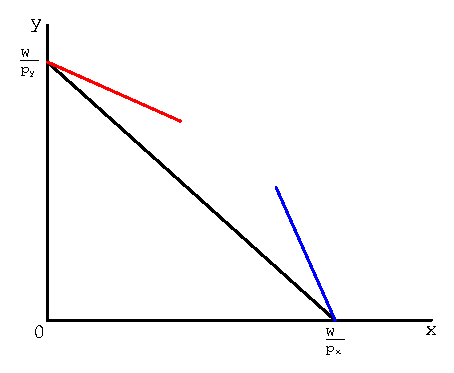
\epsfig{file=discontinuities_fig2.eps}}{\label{two}}

If the consumer's indifference curves are all flatter than the budget line,
then the solution to the maximization problem has to occur at the point $( 0,
\frac{W}{p_y} )$. Then, the consumer's indifference curves will look like the
red line. They are flatter when their slope ($- \frac{a}{b}$) is closer to zero
than $- \frac{p_x}{p_y}$, or when $\frac{a}{b} < \frac{p_x}{p_y}$. Now, we know
the entire demand curve for the consumer: demand for good $y$ is equal to
$\frac{W}{p_y}$ when $\frac{a}{b} < \frac{p_x}{p_y}$; $0$ when $\frac{a}{b} >
\frac{p_x}{p_y}$; and is anything between $0$ and $\frac{W}{p_y} $ otherwise.
You should derive this result using Lagrangian methods to see how the graphical technique is much more straightforward.

\section{Non-linear Pricing}

The main purpose of this chapter isn't to take you back to things you learned
in your first-year course. The purpose is to show you that the Lagrangian
technique is not {\tmem{the}} way to solve maximization problems, it is just
one technique that may prove useful. You will encounter problems where it
doesn't work well quite often in practise. A practise called
{\tmem{non-linear pricing}} is one example. This exotic name means that the per unit price that you pay may depend on how much you want to buy. There are two ways that
this can work. Let's look first at the case where the marginal price is
increasing. It works this way: the price of good $y$ is held constant at $1$.
The price for each of the first $n$ units of good $x$ is $p$, but if you want
to buy more than $n$ units, then each additional unit beyond $n$ will cost a
{\tmem{higher}} price $p + d p$.

Cable television companies often use this kind of pricing scheme. There is a
basic package consisting of around 50 channels. Specialty channels can be
added to the package, but a bundle of specialty channels might involve only
another 10 channels. The cost of the extra 10 channels will often be about as
high as the first 50. Apparently, tickets to World Cup soccer matches also
work this way. You can participate in a lottery, and win the right to buy a
pair of tickets to a World Cup match. If you want four tickets, however, you have to
buy the additional tickets from resellers at much higher prices.

Our consumer faces a budget line given in Figure \ref{kinked-bl}.

\tmfloat{h}{small}{figure}{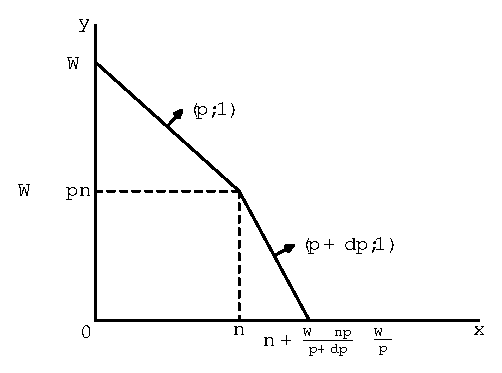
\epsfig{file=discontinuities_fig3.eps}}{\label{kinked-bl}}

The important point in the diagram is the bundle $( n, W - \tmop{pn} )$. The
line segment connecting this point with $( 0, W )$ has slope $- p$. The line
segment connecting this point to $\left( \frac{W - \tmop{np}}{p + d p}
\right)$ is steeper and has slope $- p - d p$. The arrows that point outward
from the edges of the budget set represent a convenient way to illustrate the
slope of the line segment. Notice that these arrows are perpendicular to the
line segments that they touch. You can imagine that the arrow labeled $( p, 1
)$ on the upper part of the budget set is itself a little vector in
{\tmname{{\tmname{$\mathbbm{R}^2$}}}}. The $x$-coordinate of this vector is
$p$ and the $y$-coordinate is $1$, as illustrated. This is a convenient way to
say that the slope of the line segment that the arrow is touching is $p$.

Where does the point $( n, W - \tmop{pn} )$ come from? Well, if our consumer decided to purchase exactly $n$ units of good $x$, she would spend $p n$ and have $W - p n$
dollars left over to spend on good $y$. If she decides to go further and spend
all her money on $x$, then she will have $W - n p$ dollars left over after she
buys her first $n$ units of good $x$. This will allow her to afford $\frac{W -
n p}{p + d p}$ more units of good $x$.

Let's stick with preferences of the form (\ref{cd}) so that we don't have to
worry about corner solutions. Figure \ref{more-solutions} indicates the three possible solutions to the consumer's problem.

\tmfloat{h}{small}{figure}{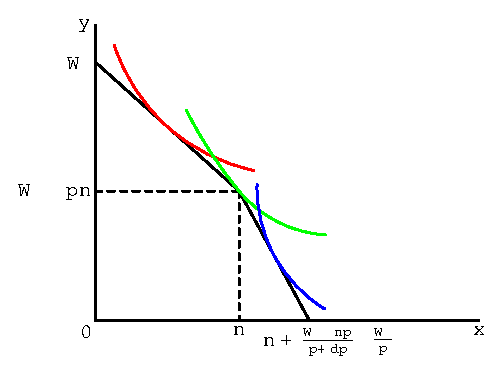
\epsfig{file=discontinuities_fig4.eps}}{\label{more-solutions}}

The highest indifference curve could be tangent on the upper section, the
lower section, or the indifference curve may not be tangent to either section
if it just touches the kink as with the green curve in the figure. In this
case, the optimal solution does not have to satisfy the first order conditions
because the constraint set is not {\tmem{differentiable}}.

Now, let's use the special properties of the utility function given by
(\ref{cd}) to give a complete solution to this problem. We will basically
whittle the problem down piece by piece until we find a solution. It is a bit
more complex than simply writing first order conditions, but still pretty
algorithmic. First, simply ask what the consumer would do if she had income
$W$ and could buy all she wanted at price $p$. There are two possibilities
here: either $\frac{\alpha W}{p} < n$ or not. You can see these two in Figure
\ref{impossible}.

\tmfloat{h}{small}{figure}{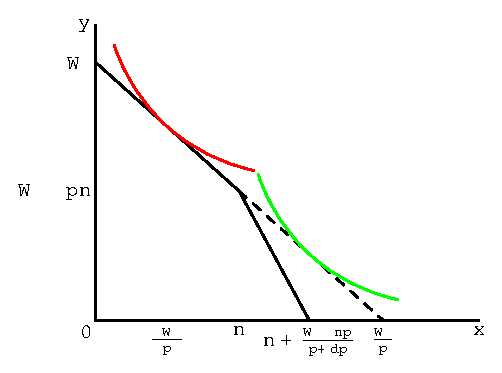
\epsfig{file=discontinuities_fig5.eps}}{\label{impossible}}

If the tangency occurs on the upper segment of the budget line (the red
indifference curve), then you are finished. The consumer will simply purchase
$\frac{\alpha W}{p}$ units of good $x$ just as she would have without the
non-linear price. On the other hand, if the tangency occurs on the dashed
segment of the budget line (the green indifference curve), then the consumer
would have liked to purchase more than $n$ units of good $x$ at the original
price. This isn't going to be feasible for her, since each unit beyond the
$n^{\tmop{th}}$ actually costs here $p + d p$.

In this case, we can try a trick. Let's take the lower segment of the budget
line and extend it so that it looks like the budget line the consumer would
face if she could buy all the good $x$ she wants at the constant price $p + d
p$. In addition, let's adjust her income so that she is able to afford exactly
$n + \frac{W - n p}{p + d p}$ units of good $x$ if she decides to spend all
her money on good $x$. This is pretty easy. To find this, just solve
\[ \frac{W'}{p + d p} = n + \frac{W - n p}{p + d p} \]
for $W' = W + n d p$. Now, solve the consumer's problem under these new
circumstances (using (\ref{cd})) and you get the choice for $x$ to be
\[ \frac{\alpha ( W + n d p )}{p + d p} \]
If this solution is larger than $n$, you are finished. As you can see from
Figure \ref{lower-part}, our consumer can't do any better by cutting
consumption of good $x$ below $n$.

\tmfloat{h}{small}{figure}{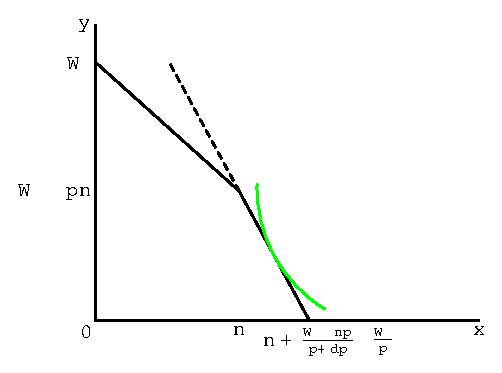
\epsfig{file=discontinuities_fig6.eps}}{\label{lower-part}}

On the other hand, if $\frac{\alpha ( W + n d p )}{p + d p} < n$ (and you have
already checked that $\frac{\alpha W}{p} > n$), then you are left with one
remaining possibility: the solution is right at the kink in the budget
line with $x^{\ast} = n$.

This gives us a pretty complete solution to the problem. The important thing
to observe is that we used the Lagrangian technique (implicitly because we
used it to solve for the demands when preferences are given by (\ref{cd})),
but only as part of a more complicated algorithm. The more complicated
algorithm became necessary because the budget set that we are dealing with has
a kind of discontinuity.

Here is a picture that very nicely summarizes the information we have learned
from this process.

\tmfloat{h}{small}{figure}{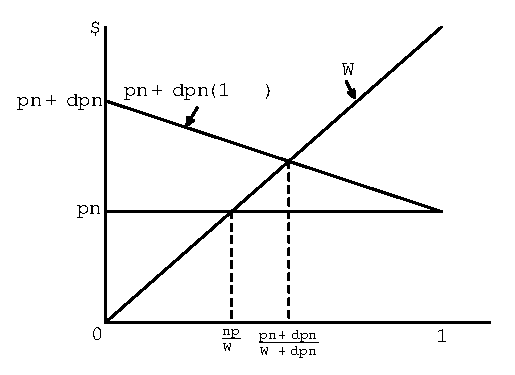
\epsfig{file=discontinuities_fig7.eps}}{}

We have determined that if $\frac{\alpha W}{p} \leqslant n$ then our consumer
will just buy fewer than $n$ units and won't have to pay the higher price.
This is like a ticket buyer who simply buys one or two tickets when he wins the
world cup lottery. This inequality is the same as $\alpha W \leqslant p n$. So,
the diagram draws the graph of the function $\alpha W$ and $p n$. The latter, of course, doesn't depend on $\alpha$ so the graph is just a
horizontal line. The point where these two functions intersect is $\frac{n
p}{W}$ as is shown in the diagram.

We also figured out that if $\frac{\alpha ( W + n d p )}{p + d p} > n$, then
our consumer would buy strictly more than $n$ units, paying the lower price
$p$ for the first $n$ units, then shelling out the higher price for the
others. This is like the soccer fan who buys additional higher-priced tickets from
resellers (scalpers).

This inequality is the same thing as $\alpha ( W + n d p ) > n ( p + d p )$ or
$\alpha W > n p + ( 1 - \alpha ) n d p$. The figure adds the graph of the
function $n p + ( 1 - \alpha ) n d p$ which is the downward sloping curve. As
you can see, this curve starts out above $p n$ and eventually equals it. This
curve intersects $\alpha W$ at the point $\frac{p n + n d p}{W + n d p}$ as
marked in the Figure. So, in the interval between $\frac{n p}{W}$ and $\frac{p
n + n d p}{W + n d p}$, our consumer buys exactly $n$ units of the good.

Perhaps from this analysis, you can tell why firms will use non-linear prices.
The people who choose to buy $n$ or fewer units don't care what price you
charge for extra units of output, because they don't buy any extra. That means
that you can raise the price you charge your fanatic customers without losing
any business from those who are a little less fanatical.

\section{Sign-up Fees}

Another common pricing technique is the sign-up fee. Long distance-phone charges
work this way: you pay a fixed fee for $100$ free minutes. Each minute thereafter
will cost you an extra 5 cents. You may want only 50 minutes of long distance
service, but you will still be forced to pay the same fixed fee.

So, let's consider a sign-up fee problem.  Let's begin by fixing notation. As before, we will assume that every unit of good $y$ has
the same per unit price of \$ $1$. The sign-up fee for delivery of good $x$ will
be $K$, which will provide $n$ units of good $x$. Each additional unit of good
$x$ will cost $p$. The budget set the consumer faces in this case is given in
Figure \ref{fixed-fee}.

\tmfloat{h}{small}{figure}{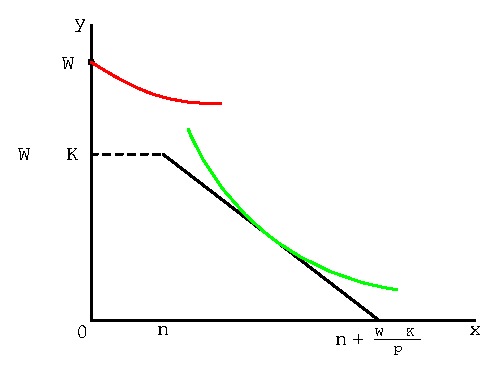
\epsfig{file=discontinuities_fig8.eps}}{\label{fixed-fee}}

Now, if the consumer only wants to buy good $y$, then she can afford $W$ units.
If her indifference curves look like the red curve that cuts through the point
$( 0, W )$, then she will do exactly that. If she wants to buy any good $x$ at
all, she must pay the fixed fee $K$. This will cause her budget set to jump
down discontinuously to the point $( 0, W - K$). She would never choose this
point if she likes good $x$ because she can have up to $n$ free units of the
good once she has paid the fixed fee. So, her budget set must also shift
discontinuously, up to the right, to the point $( n, W - K )$. If she wants more
than $n$ units of good $x$, then she will choose a tangency point on the
downward-sloping portion of the budget line (whose slope is $- p$).

Let's suppose first that our consumer has preferences given by (\ref{cd}). Then,
we can use the method we used for the last problem: combining the Lagrangian
with a systematic scan of the possibilities. To do this, let's first pretend
that the consumer simply has a fixed income equal to $W - K + n p$, and that
she can buy all the good $x$ she wants, even small amounts of it, at price
$p$. Applying the Lagrangian method with preferences given by (\ref{cd}), we
get demand equal to $\alpha ( W - K + p n ) / p$. If this is larger than $n$,
then we are finished and have found the solution to the problem. If it is less
than $n$, it means the solution is not feasible given the firm's pricing
scheme. When preferences are given by (\ref{cd}), we know that the consumer
will never choose $0$ units of good $x$. So if $\alpha ( W - K + p n ) / p
\leqslant n$, our consumer will simply choose $n$ units of good $x$.

It may be apparent to you that this pricing scheme helps the firm because it
induces some consumers who would have purchased fewer than $n$ units at a
constant price $p$ to increase the amount they buy to $n$. Of course, firms
always tout their pricing schemes as being designed to allow consumers to
choose the plan that is best suited to their needs. Perhaps, our analysis indicates
that this claim typically means best suited to the {\tmem{firm's}} needs.

To make the argument in a little stronger way, suppose that our consumer has a
slightly different utility function given by $u ( x, y ) = y + \log ( x )$.
This is a special case of the famous quasi-linear utility function that is now
just about the most widely used utility function in economics.{\footnote{You
may not see this utility function much for a while. It is most widely used in
the theory of auctions and mechanism design.}} Let's use the Lagrangian method
to figure out our consumer's demand function in this case.

She is trying to solve the problem
\[ \max_x y + \log ( x ) \]
subject to the usual constraints
\[ p x + y - W \leqslant 0 \]
\[ - x \leqslant 0 \]
\[ - y \leqslant 0 \]
The first order conditions are
\[ \frac{1}{x} + \lambda_1 p - \lambda_2 = 0 \]
\[ 1 + \lambda_1 - \lambda_3 = 0 \]
along with the three complementary slackness conditions. Since $\log ( 0 )$ is
undefined (or equal to $- \infty$), we know our consumer will always choose a
strictly positive amount of good $x$. So, by the complementary slackness
condition, $\lambda_2$ must be equal to zero. Let's suppose for the moment,
that the optimal $y$ is also positive. Then, from the first order conditions,
$x = \frac{1}{p}$. This is an odd property of quasi-linear functions, as long
as $W > 1$, the consumers demand will be independent of her income. Cigarettes
are a commodity (I can't really call them a good) that have this property for
low income people.{\footnote{Though, as income rises cigarette demand eventually
falls. Cigarette demand is also very insensitive to price changes, at least
when income is low.}}

So, let's look at the entry fee problem using this result. The next figure just
reproduces the last one with this extra information about quasi-linearity.

\tmfloat{h}{small}{figure}{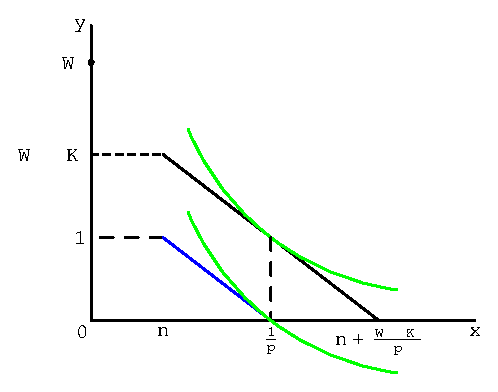
\epsfig{file=discontinuities_fig9.eps}}{}

The picture is drawn so that the consumer initially has income $W > 1$ and so
chooses to buy $\frac{1}{p}$ units of good $x$. Our Lagrangian analysis says
that if the fixed fee varies a little bit, the consumer continues to purchase
exactly $\frac{1}{p}$ units of good $x$.

Then, as we raise the fixed fee $K$, this will have no effect on our
consumer's demand for good $x$. Of course, the revenue that the firm gets
selling good $x$ to this consumer consists of $p x$ and the fixed fee, so the
firm's profit is rising as it raises the fee. If the firm raises the fixed fee
to $W - 1$, the consumer's budget line (when she pays the fixed fee) will shift
down until it is equal to the blue line in the figure. This line which connects the
point $( 0, 1 )$ to the point $( \frac{1}{p}, 0 )$. Then, our consumer will
still buy $\frac{1}{p}$ units of output, but will now give all the rest of her
income to the firm as well. When demand is insensitive to changes in consumer
income, an entry fee is a good way for a firm to raise its revenues.

You should make sure you that work out on your own what would happen if the firm
continued to raise the fixed fee beyond $W - 1$.

\end{document}
